\lab{Application}{Newton's Method, Julia Sets and Basins of Attraction}{Newton's Method}
\label{lab:NewtonsMethod}
\objective{Understand Newton's Method. Understand definition of basin of attraction.  Basic understanding of Julia Sets.}

One important technique in technical computing is Newton's method.
The goal of Newton's method is to find $\overline{x}$ such that $f\left(\overline{x}\right) = 0$.
This method is especially important in optimization, where our goal is to find minima and maxima of functions.
Newton's method is an iterative method.
In one dimension, it is defined as follows:
\[
x_{n+1} = x_n - \frac{f(x_n)}{f'(x_n)}
\]

Essentially Newton's method approximates a function by its tangent line, and then uses the zero of the tangent line as the next guess for $x_n$.

\begin{figure}[h]
\centering
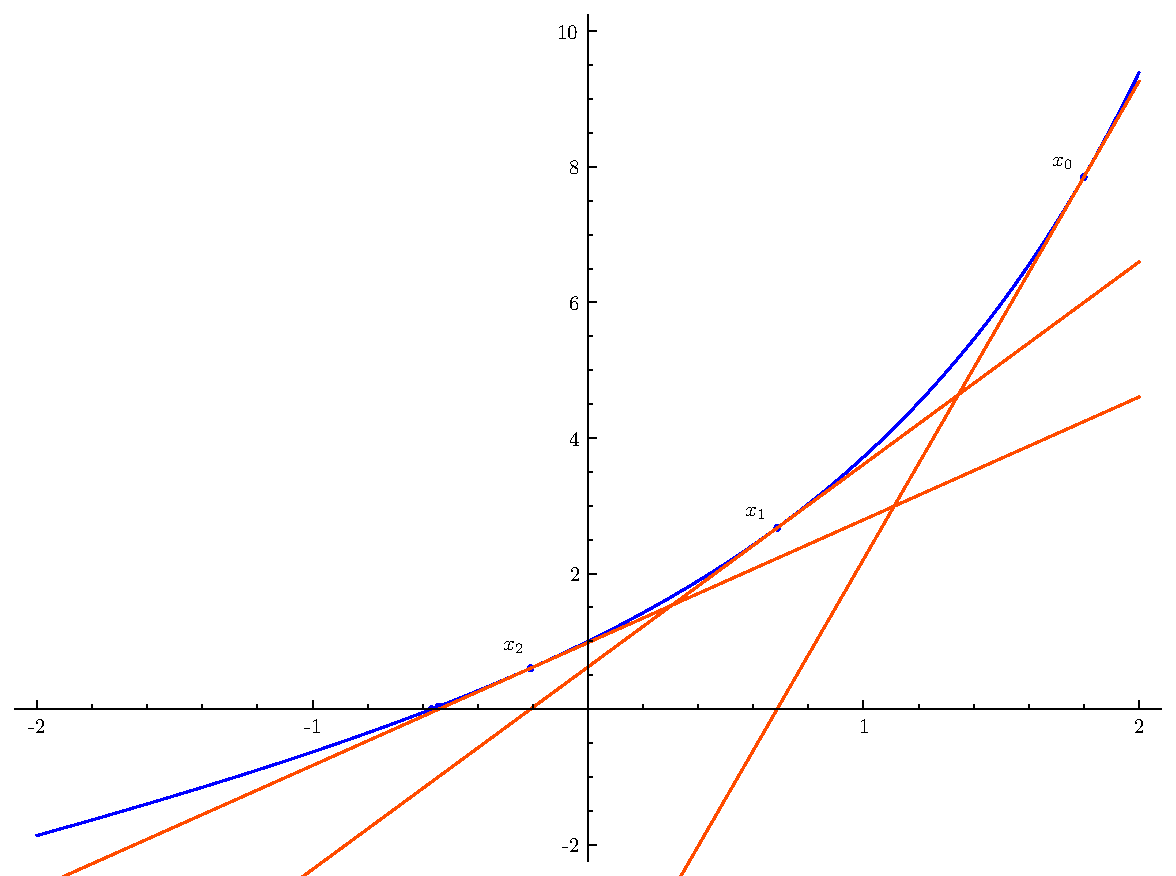
\includegraphics[width=\textwidth]{newton_iters}
\caption{An illustration of how one iteration of Newton's method works}
\end{figure}

Newton's method is powerful because of the speed of convergence.
In many cases Newton's method converges to the actual root quadratically, meaning that the error term is squared at every iteration.
This fast convergence makes it a very powerful algorithm.

Newton's method does suffer from the flaw that its convergence is dependent upon an initial guess.
If the initial guess is not sufficiently close the convergence can be much slower, or may never occur.
There are even certain pathological functions for which newton's method will never converge.

\begin{problem}
\label{prob:newton_arr}
Write a Newton's method function that runs whether or not the user inputs a derivative function.
In python this can be done by defining the derivative function as a keyword argument that defaults to \li{None}.
Also accept a maximum of how many iterations it will run and a tolerance used for the stopping condition.
Return a tuple with the computed value and boolean value telling whether it converged or not.

Compare the performance of Newton's method when you input the derivative and when you don't.
How well does each converge?
Which runs faster?
Try the following functions:

\begin{itemize}
\item $cos(x)$
\item $x^2sin(\frac{1}{x})$
\item $(\frac{sin(x)}{x})-x$
\item $x^2-1$
\item $x^3 - x$
\end{itemize}

For the last two, look at the results of the iteration on equispaced points between -2 and 2.
Which points converge to which roots?

There are also examples of when Newton's Method does not converge.
Test your newton's method function on $x^{1/3}$.
Have it test at eqispaced starting points on a given interval and return the corresponding values after a given number of iterations.
What do you see?
\end{problem}

\begin{comment}
\begin{problem}
Extend your Newton's method even further so that it will work on systems of equations.
Suppose that $F: \mathbb{R}^n \rightarrow \mathbb{R}^n $.
The relevant equation is
\[
x_{i+1} = x_i - J^{-1}F(x_i)
\]
Note that you should not calculate the inverse Jacobian.
\li{scipy.linalg.solve(A,b)} gives you the solution $x$ to the equation $Ax=b$.
Use this fact to calculate $J^{-1}F$ from $J$ and $F$.
You should be able to make this function work whether or not the user inputs a Jacobian.
This also means that you will have to use your own \li{jacobian} function.
\end{problem}
\end{comment}

\section*{Basins of Attraction and Julia Sets}
Thus far we have only noted the fact that Newton's method converges under good circumstances.
Another topic of interest is determining which starting values converge to which roots.
An plot showing which points converge to which roots for the function $x^2 + x - 2$ is shown in Figure \ref{Fig:basins1}.

\begin{figure}
\begin{center}
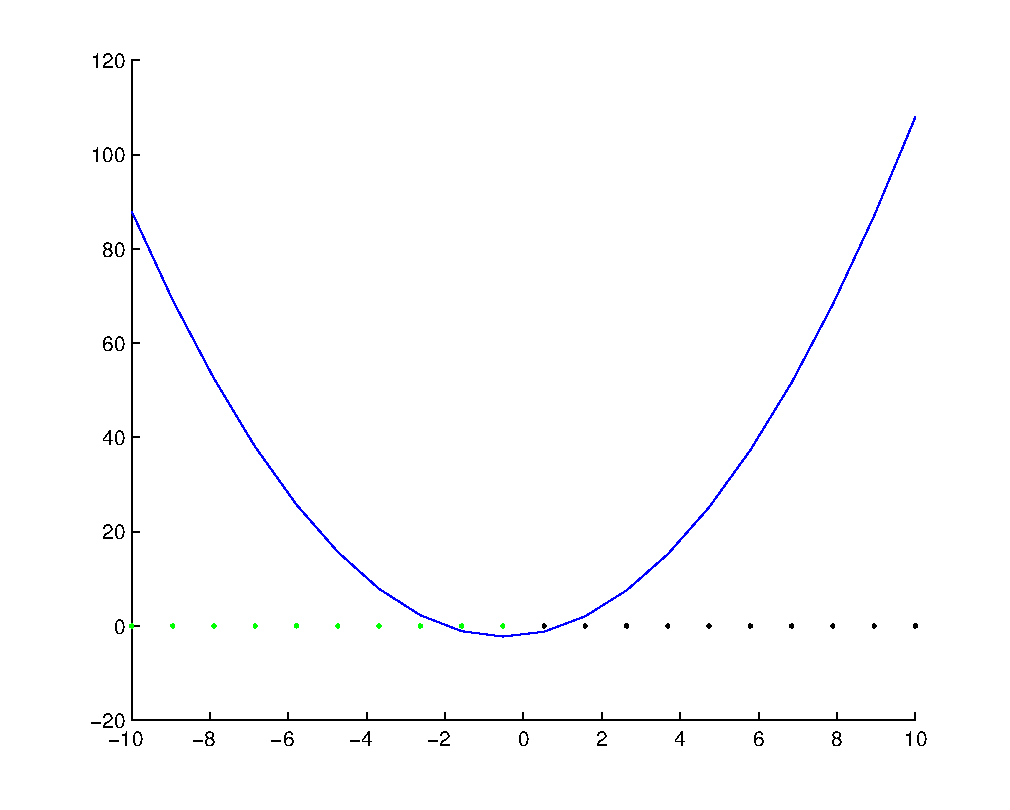
\includegraphics[scale=0.5]{basins1}
\caption{The plot of $f(x) = x^2 + x - 2$ along with 20 seed values for Newton's Method.
The green values all converge to the root at -2, and the black values will converge to the root at 1.}
\label{Fig:basins1}
\end{center}
\end{figure}

It turns out that for $f(x) = x^2 + x - 2$, any seed value will converge to one root or the other.
We call the set of points that converge to a single value through an iterative process a basin of attraction.
We can see in Figure \ref{Fig:basins1} a set of seed values that are color coded to indicate which root they converge to with Newton's method.

We now extend these ideas to complex functions.
There is an entire field of mathematics devoted to the study of such functions, but here we only examine some basic properties as they pertain to the generation of Julia sets.
Like other functions we have thus far been exposed to, a complex function maps an input to a unique output.
However, in this case both the input and the output come from the space of complex numbers.

Given a sufficiently ``nice'' complex function, we can apply Newton's method in a similar way to how we applied it in the real case.
However due to the nature of the space we are mapping from and to, we no longer have access to the intuitive visual representations of functions that we saw in the real case.
We can, however, graph the basins of attraction for Newton's method on the complex plane.
For example, let:
\[
f(z) = z^2 - 1
\]
Derivatives for nice complex functions behave much the same way as in the real case:
\[
f'(z) = 2z
\]
It is straightforward to verify that $f$ has two roots at 1 and -1.

In order to better visualize basins of attraction in the complex plane we will use the function li{pcolormesh} from the pyplot library in matplotlib.
The following is an example of how to use this function.
It allows us to color different portions of a plane according to the value of a function at each point.

\begin{lstlisting}
import scipy as sp
from matplotlib import pyplot as plt
n=401
x=sp.linspace(-2,2,n)
y=sp.linspace(-2,2,n)
X,Y=sp.meshgrid(x,y)
def func(x):
    return sp.real(x**3-2*x**2-x+2)
C=func(X+complex(0,1)*Y)
plt.pcolormesh(X,Y,C)
plt.show()
\end{lstlisting}

\begin{problem}
Modify your code from Problem \ref{prob:newton_arr} to graph the basins of attraction for a polynomial in the complex plane.
Examine the basins of attraction for the following complex functions on the following domains.
\begin{itemize}

\item $z^3 - 2 z^2 - 2 z + 2$ on the set of complex numbers $a + b i$ such that $a \in \left[-\frac{1}{2}, 0\right]$ and $b \in \left[-\frac{1}{4}, \frac{1}{4}\right]$.

\item $3 z^3 - 2 z^2 - 2 z + 2$ on the set of complex numbers $a + b i$ such that $a \in \left[-1, 1\right]$ and $b \in \left[-1, 1\right]$.

\item $z^4 + 3 z^3 - 2 z^2 - 2 z + 2$ on the set of complex numbers $a + b i$ such that $a \in \left[-1, 1\right]$ and $b \in \left[-1, 1\right]$.

\item $z^3 - 1$ on the set of complex numbers $a + b i$ such that $a \in \left[-1, 1\right]$ and $b \in \left[-1, 1\right]$.

\end{itemize}
Be aware that Newton's method may not converge for every point in these intervals, so you will have to manually set the pixels that result in a value of \li{nan} to something else.
One good approach is to set the roots of the polynomial to numbers $0, 1, \dots, k$ and then set the values of \li{nan} to $k+1$.

Make sure that when plotting you start with low resolution.
Even if you generate a plot using an array of $100$ by $100$ points, you will be running Newton's method on your test function $10,000$ times, so be careful.
\end{problem}

Another well-studied fractal in the complex plane is the Mandelbrot set.
It is defined as the points $c \in \mathbb{C}$ for which the sequence
\[z_n = z_{n-1}^2 + c\]
is bounded.

\begin{problem}
Generate another grid of complex numbers on $[-1.5,.5]\times[-i,i]$.
Consider the recurrence relation $x_n = x_{n-1}^2 + c$.
Run this iteration 30 times with a resolution of $200 \times 200$ and display the plot.
\end{problem}
